
\chapter{Sviluppo applicazioni web}


da fare

%
% Commento: questa � la prima sezione
%
\section{Web 1.0}

\index{?}

Il Web \'e il principale servizio offerto da Internet e permette di consultare un elevato numero di contenuti e allo stesso tempo dei servizi messi a disposizione da altri utenti della rete.

Si basa principalmente su 3 componenti:

\begin{enumerate}


\item html:il linguaggio di markup per le pagine web.

\item http:un protocollo di rete che permette lo scambio di informazioni.

\item url:l'indirizzo che contraddistingue in maniera univoca una risorsa.


\end {enumerate}

La prima idea di web f\'u teorizzata da Vanner Busgh nel 1945, ma solo nell'agosto 1991 Tim Berners-Lee pubblic\'o il primo sito internet della storia, con l'obbiettivo di favorire la condivisione di documenti tra i ricercatori.
Divenne quasi subito popolare e numerose entit\'a commerciali inziarono ad investire grandi quantit\'a di denaro nello sviluppo e nella progettazione di siti web.
In quel periodo il paradigma utilizzato per la programmazione dei siti prevedeva un'interazione unilaterale,cio\'e forniva all'utente solamente la possibilit\'a di scegliere e visualizzare i contenuti messi a disposizione da altri, ma non di modificare in alcun modo lo stato o le informazioni.
I file erano in formato html e non era prevista alcuna modifica o manipolazione da parte del server prima dell'invio del file al browser dell'utilizzatore, da qui il nome web statico.


\subsection{HTML}

Html \'e un linguaggio di markup proposto da Tim Berners-Lee nel 1989 per la formattazione e l'impaginazione dei documenti ipertestuali.
Questo linguaggio definisce il layout della pagina web tramite l'utilizzo di particolari tag di formattazione, i quali hanno lo scopo di specificare la funzione, il colore, la grandezza e la dimensione della porzione di testo da essi delimitata.
\begin{figure}[tp]
    {\begin{center}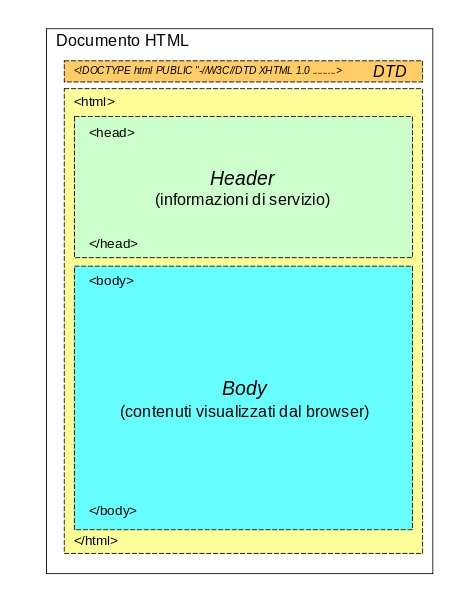
\includegraphics[width=8cm]{figure/Struttura_html.jpg}\end{center}}
\caption{Struttura di una pagina html\label{struttura_html}}
\end{figure}
Come si pu\'o notare nella figura ~\ref{struttura_html}, il file html deve iniziare con una stringa che indica il tipo di sintassi e la versione in cui \'e stato scritto il documento per poter garantire la corretta visualizzazione da parte del browser.
La struttura pi\'u esterna \'e contenuta nei tag <html> e </html> e comprende obbligatoriamente due sottosezioni:head e body.
Head contiene tutte le informazioni di controllo che non sono visualizzate dal browser, mentre body contiene quelle che l'utilizzatore pu\'o vedere a schermo. 
Dentro queste due sottosezioni \'e possibile utilizzare ulteriori tag per effettuare controlli o per specificare la formattazione dei contenuti.
\begin{figure}[tp]
    {\begin{center}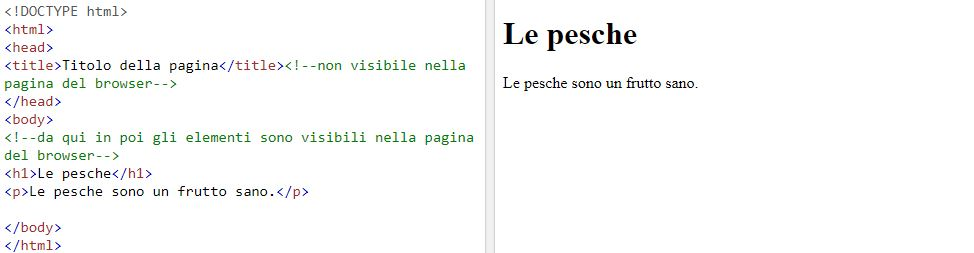
\includegraphics[width=18cm]{figure/codice_HTML.jpg}\end{center}}
\caption{Esempio di una pagina html.\label{codice_html}}
\end{figure}

Nella figura ~\ref{codice_html} si pu\'o notare come i tag dentro la sezione Head non siano direttamente visibili nella pagina caricata dal browser, al contrario di quelli contenuti in body, i quali vengono visualizzati.

\subsection{Protocollo http}


Il protocollo HTTP (HyperText Transfer Protocol) \'e di tipo applicativo e viene utilizzato per il trasferimento di informazioni sul web nell'architettura client-server, nella quale il server resta solitamente in ascolto sulla porta 80.
La prima versione (0.9) fu pubblicata negli anni '80, ma la prima versione effettivamente disponibile (1.0) fu sviluppata sempre da Tim Berners-Lee nell'anno 1991.
La prima versione era molto limitata, non prevedeva infatti la possibilit\'a di ospitare pi\'u di una risorsa all'interno del server, era priva di meccanismi di sicurezza e non potevano essere riutilizzate le connessioni aperte; tutto questo port\'o alla sua evoluzione (versione 1.1) nel 1999.

Il protocollo http si basa su un meccanismo di richiesta da parte del client (solitamente il browser) e di risposta da parte del server (solitamente la macchina su cui \'e ospitata la risorsa), tanto che sono previsti solo due tipi di messaggi:uno per la richiesta e uno per la risposta.
Le connessioni vengono solitamente chiuse dopo il ricevimento della risposta garantendo un numero limitato di connessioni attive contemporaneamente, ma svantaggiando lo sviluppo di servizi web con meccanismi di sessione.
Questo difetto fu poi risolto implementando i coockie che, con le dovute configurazioni, permettono di conservare lo stato della sessione dell'utente anche con un protocollo stateless come l'HTTP.

\subsection{URL}

Con il termine URL (Uniform Resurce Locator) si intende la sequenza di caratteri che identifica in maniera univoca una risorsa nella rete.
La struttura dell' URL si compone solitemente di 7 parti:



protocollo://[username:password@]host[:porta]/percorso[?querystring][\#fragment]

\begin{enumerate}
\item Specifica il protocollo da utilizzare nel dialogo con il server, di dafault \' HTTP.
\item \'E possibile indicare le credenziali per l'accesso alla risorsa richiesta; alcuni browser impediscono questi parametri a causa del basso livello di sicurezza. L'username e la password infatti vengono trasmesse in chiaro e l'utilizzatore potrebbe diventare vittima di phishing.
\item L'host identifica il server sul quale \'e ospitata la risorsa e pu\'o essere rappresentato usando l'indirizzo IP o indicando il nome di dominio; nel secondo caso il browser si occuper\'a di convertirlo in IP attraverso il DNS.
\item Indica la porta del servizio di rete al quale si vuole effettuare la richiesta; di default \'e 80 per il protocollo HTTP e 443 per il protocollo HTTPS.
\item Indica il percorso nel file system del server in cui giace la risorsa che si desidera ricevere; se non viene specificato il server restituir\'a un percorso impostato di default.
\item \'E possibile inserire una serie di stringhe separate dalla parte precedente dal simbolo "?" che consentono l'invio al server di informazioni extra da parte del client
 (es. ...?parametro1=valore\&parametro2\=valore2)
\item Indica una parte o una porzione della risorsa.

\end{enumerate}

\section{Web 2.0 e applicazioni multipagina}

\index{?}

Il paradigma di sviluppo descritto nella sezione precedente risulta poco pesante per il server che non dovr\'a eseguire alcuna attivit\'a computazionale dal momento che non avviene nessuna modifica dei contenuti inviati all'utente.
Nonostante le buone performance, questo paradigma soffre di un numero elevato di limiti, come l'impossibilit\'a di permettere all'utente di interagire con la pagina o di adeguare le informazioni da inviare in base all'utilizzatore che le richiede.
Queste mancanze portarono molti siti web statici alla migrazione verso il paradigma dinamico.

Per permettere al server di generare pagine html in maniera dinamica furono inizialmente sviluppate le CGI (Common Gateway Inteface) con le quali era possibile delegare ad un programma esterno la generazione in tempo reale del codice html, anche se con limitazioni e risultando una pratica molto pesante per il calcolatore.
Negli anni successivi i browser divennero sempre pi\'u completi di funzionalit\'a come il supporto dei linguaggi di scripting e nei web server si inziarono ad utilizzare linguaggi ideati per la creazione di pagine dinamiche; il web era diventato una possibile piattaforma sulla quale sviluppare vere e proprie applicazioni.


\subsection{HTML5}

%\begin{figure}[tp]
%    {\begin{center}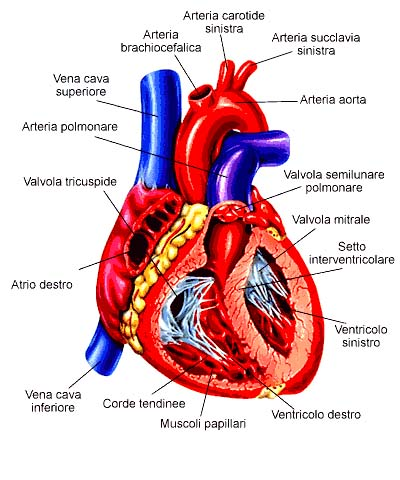
\includegraphics[width=8cm]{figure/cuore_aperto.jpg}\end{center}}
%\caption{Il cuore  \label{cuore}}
%\end{figure}

Il web dinamico, comunemente chiamato web 2.0, non potrebbe esistere senza HTML5 che ha introdotto numerose novit\'a allo scopo di mettere a disposizione degli sviluppatori un'insieme di funzionalit\'a per la creazione di pagine web dinamiche e non pi\'u statiche.
In particolare, questa nuova versione, prevede la possibilit\'a di salvare in locale una quantit\'a elevata di dati fino a permettere l'utilizzo di un' applicazione web anche in assenza momentanea di connessione.

Grazie a queste nuove novit\'a ci fu un notevole aumento di web app sviluppate unendo HTML5, css e JavaScript; questi 3 linguaggi infatti assieme riescono a fornire tutte le funzionalit\'a richieste per lo sviluppo di una generica applicazione:HTML5 rappresenta il formato delle pagine e il suo contenuto, css gestisce gli aspetti presentazionali e l'estetica della pagine e JavaScript gestisce le interazioni dell'utente.

\subsection{CSS}


Prima dell'arrivo di css l'unico modo che aveva lo sviluppatore per modificare la formattazione delle proprie pagine html era quello di sfruttare i tag proprietari forniti dai browser.
Questi tag per\'o risultavano spesso pesanti, ridondanti e incompatibili con gli altri browser, soprattutto con i dispositivi mobile; questo causava la visualizzazione sul browser di una pagina mal formattata, confusa e di difficile lettura.
Per tentare di risolvere tali problemi, nel 1996 W3C eman\'o le specifiche della prima versione di CSS, con l'obbiettivo di separare il contenuto della pagina dalla sua formattazione, riuscendo a risolvere almeno in parte i problemi sopra descritti.
Le successive versioni permisero di creare fogli di stile separati per i dispositivi mobili garantendo una buona compatibilit\'a anche con questi device pi\'u recenti.

\subsection{JavaScript}

JavaScript \'e un linguaggio di scripting interpretato, debolmente orientato agli oggetti e tipizzato, comunemente utilizzato nella programmazione web lato client per la creazione di siti e applicazioni web.
\'E in grado di creare effetti dinamici sulla pagina tramite funzioni invocate da eventi scatenati dalle interazioni dell'utente, come il click del mouse.
Fu da subito molto apprezzato per la sua semplicit\'a, per la sua natura di linguaggio asincrono e perch\'e soddisfava in pieno le esigenze delle prime applicazioni web.

Recentemente si utilizza anche lato server grazie a Node.js, una piattaforma event driven sviluppata quasi interamente in javascript, che offre un alto livello di efficienza grazie al suo modello di networking. Quest'ultimo non sfrutta la programmazione concorrente, ma rimane in sleep fino al verificarsi di un evento immediatamente gestito, eventualmente in maniera asincrona.


Le caratteristiche principali di JavaScript sono le seguenti:

\begin{enumerate} 

\item \'e un linguaggio interpretato,quindi il codice non deve essere compilato, ma viene eseguito dall'interprete incluso nel browser in run time incaricando quindi il client di effettuare le operazioni computazionali necessarie alleggerendo di conseguenza il server.

\item la sintassi \'e simile a quella di c e java

\item \'e un linguaggio debolmente tipizzato

\item \'e un linguaggio debolmente orientato agli oggetti

\end{enumerate} 
Per lo sviluppo delle prime applicazioni basate sul web, javascript fu molto apprezzato per le sue caratteristiche, ma con il continuo aumento di complessit\'a delle applicazioni basate sul web si \'e sentita la neccessit\'a dello sviluppo di framework che aiutassero il programmatore nell'organizzazione del codice.

\subsection{AJAX}

Con il termine AJAX (Asynchronous JavaScript and XML) si intende una tecnica multipiattaforma di sviluppo di applicazioni web dinamiche e interattive che permette uno scambio di dati tra client e server asincrono e in background.
Questa tecnica \'e alla base dello sviluppo delle applicazioni che usano il web come piattaforma perch\'e permette la modifica della pagina senza che il browser debba effettuare un'operazione di refresh.

Per poter eseguire le operazioni di scambio dati in background si sfruttano le funzionalita offerte dai linguaggi di scripting come JavaScript, mentre per il markup e lo stile ci si appoggia a HTML e CSS.
A differenza di come suggerisce il nome,i dati scambiati possono essere in vari formati e non necessariamente in XML,infatti \'e possibile trasferire degli oggetti in formato JSON o del semplice testo in HTML.

\begin{figure}[tp]
    {\begin{center}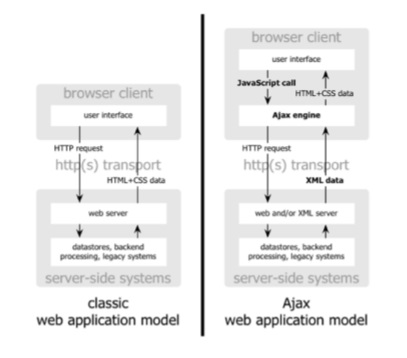
\includegraphics[width=12cm]{figure/ajax.jpg}\end{center}}
\caption{Differenze tra l'utilizzo di ajax o del metodo classico   \label{ajax}}
\end{figure}

La figura ~\ref{ajax} mostra come AJAX funga da intermediario in grado di gestire le richieste del client e le risposte del server; le prime vengono scatenate da una chiamata in JavaScript, mentre le seconde vengono ricevute come dati di tipo XML(o altri formati) dai quali viene generato il codice HTML e CSS.

Per poter essere correttamente utilizzate, le applicazioni web sviluppate con AJAX devono essere eseguite su browser che supportino tutte le tecnologie sopraelencate, ma al giorno d'oggi sono interamente supportate da tutti i dispositivi, compresi i device mobili.
Grazie a AJAX divent\'o possibile sviluppare applicazioni che stessero interamente in una sigola pagina web, delegando ai linguaggi di scripting l'onere di modificare le informazioni visualizzate sul browser tramite l'utilizzo delle comunicazioni asincrone e in background con il server.




\section{Singole Page Application}

\index{?}

Con il termine spa (single page application) si intende un'applicazione web contenuta interamente in una pagina al fine di migliorare la user experience fino a rendere l'esperienza paragonabile all'utilizzo di un'applicazione desktop.
A differenza delle applicazioni desktop, le spa sono molto facili da aggiornare, dal momento che basta caricare sul server l'ultima versione senza costringere l'utente a reinstallare il programma.
Le applicazioni multipagina richiedono il refresh quasi ad ogni interazione con la pagina, generando quindi dei tempi di attesa maggiori rispetto ad una spa. 
Con questo ultimo tipo di programmazione della pagina, invece, si \'e in grado di ottenere un'applicazione molto veloce (solo il caricamento inziale diventa leggermente pi\'u lungo) e l'utilizzo della banda \'e solitamente limitato all'accesso ai dati, che spesso sono contenuti in database remoti.
Per ridurre ulteriormente l'uso di banda si pu\'o optare per il salvataggio in cache dei dati,se il tipo di applicazione lo permette, al fine di limitare gli accessi al database e di conseguenza ridurre i tempi di caricamento necessari al corretto funzionamento dell'applicazione.

Come si pu\'o notare nelle figure ~\ref{applicazione_multipagina} e ~\ref{applicazione_singola_pagina}, un'altra differenza rispetto alla programmazione multipagina riguarda l'utilizzo dei file html: nella spa non si avranno pi\'u molte pagine html complete, ma se ne avr\'a una contenente i placeholders i quali saranno successivamente riempiti dinamicamente tramite le funzioni messe a disposizione da JavaScript.
\begin{figure}[tp]
    {\begin{center}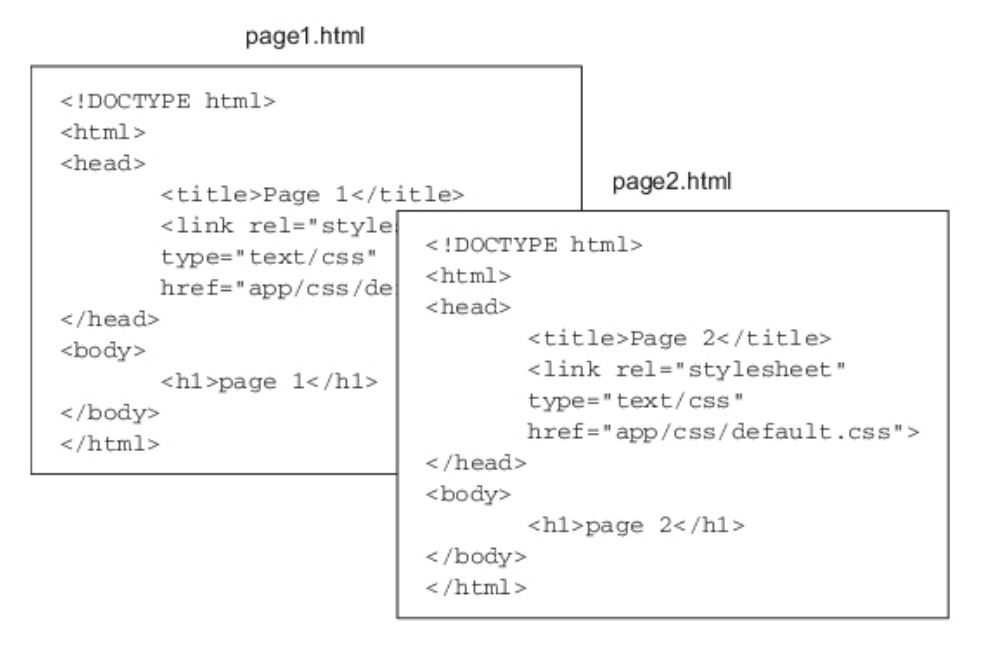
\includegraphics[width=12cm]{figure/applicazione_multipagina.jpg}\end{center}}
\caption{Struttura html di un'applicazione multipagina  \label{applicazione_multipagina}}
\end{figure}
\begin{figure}[tp]
    {\begin{center}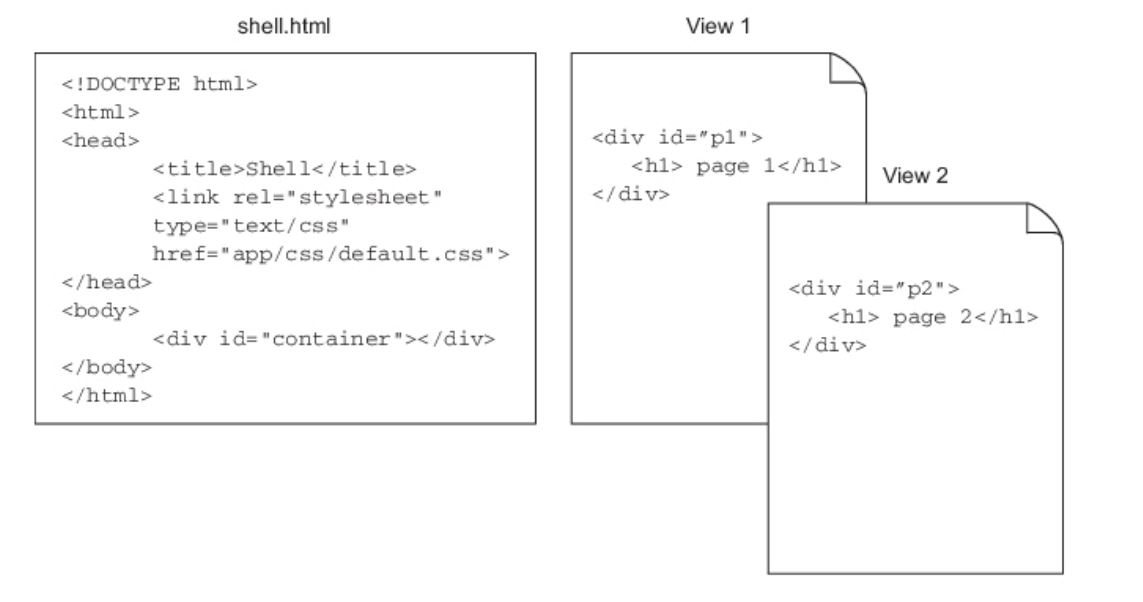
\includegraphics[width=12cm]{figure/spa.jpg}\end{center}}
\caption{Struttura html di una single page applicatione\label{applicazione_singola_pagina}}
\end{figure}


Con l'avanzare del tempo le applicazioni web sono diventate sempre pi\'u complesse e gli sviluppatori hanno avvertito la necessit\'a di framework che li aiutassero nell'organizzazione e nella stesura del codice per evitare risultati caotici e facilitare il riutilizzo e la manutenzione nel tempo.
